\documentclass[conference]{IEEEtran}
\IEEEoverridecommandlockouts
\usepackage[T1]{fontenc}
\usepackage{mathptmx}
\usepackage{cite}
\usepackage{amsmath}
\usepackage{graphicx}
\usepackage{booktabs}
\usepackage[hidelinks]{hyperref}
\newcommand{\usd}{\$}
\makeatletter\newcommand{\tabinput}[1]{\@@input #1 }\makeatother
\newcommand{\maxcovstd}{0.004}
\newcommand{\kappafit}{4.0}

\DeclareMathOperator*{\median}{median}

\begin{document}

\title{Mondrian and Residual-Weighted Conformal Uncertainty Bands for Physics-Informed American Option Pricing}

\author{\IEEEauthorblockN{Gaurang Gupta}
\IEEEauthorblockA{MPSTME, SVKM's NMIMS\\Mumbai, India\\
GAURANG.GUPTA10@nmims.in}
\and
\IEEEauthorblockN{Arush Gupta}
\IEEEauthorblockA{MPSTME, SVKM's NMIMS\\Mumbai, India\\
ARUSH.GUPTA53@nmims.in}
\and
\IEEEauthorblockN{Utkarsh Nigam}
\IEEEauthorblockA{MPSTME, SVKM's NMIMS\\Mumbai, India\\
UTKARSH.NIGAM54@nmims.in}}

\maketitle

\begin{abstract}
Physics-informed neural networks (PINNs) can price options without labelled prices, but a point price is not a risk number. We study split conformal prediction on top of PINN pricers for European and American puts under geometric Brownian motion, with exact Black-Scholes and 500-step binomial prices as calibration and test labels. Over ten training seeds, the PDE loss cuts the European mean absolute error from \usd 4.42 (a control without the PDE term) to \usd 0.25 and shrinks the 90\% split-conformal band from \usd 19.43 to \usd 0.94. With 3000 labels, eight of ten labelled regressors are more accurate inside their training region, but kernel and polynomial ridge fail outside it. Split conformal reaches nominal marginal coverage for every model. A fix to a weak complementarity penalty cuts the American PINN's bias to \usd 0.22 but adds calendar violations (16.8\% of pairs). The raw PDE residual is uninformative for the American put (rank correlation 0.01) and widens the band. The complementarity residual $\min(L[u],u-h)$ is a better score (rank correlation 0.38; band \usd 1.13 against \usd 1.97), but plain split is narrower (\usd 0.93). Mondrian buckets give the narrowest band (\usd 0.85) and the best worst-bucket coverage (0.86 against 0.66). All labels are synthetic; we claim no market coverage.
\end{abstract}

\begin{IEEEkeywords}
physics-informed neural networks, American options, conformal prediction, uncertainty quantification, no-arbitrage
\end{IEEEkeywords}

\section{Introduction}
A trader who receives a model price also needs to know how far that price may be from the truth. A price without a band is not a risk number. An American contract adds a second difficulty. Its holder can exercise early, the exercise boundary has to be found as part of the solution, and no closed-form price exists \cite{merton1973theory,hull2022options}. Trees and Monte Carlo produce accurate reference values \cite{cox1979option,longstaff2001valuing}. They cannot tell us, however, the error of a fast surrogate at an unseen point. Learned pricers bring two further issues. Regressors trained on labelled prices need many labels and can break calendar or convexity conditions. PINNs need no labels \cite{raissi2019physics}, but their error is not known in advance.

This paper puts distribution-free conformal bands \cite{vovk2005algorithmic,lei2018distribution} around PINN pricers and asks which difficulty score should scale the band. Our contributions are as follows.
\begin{enumerate}
\item A controlled study of split, residual-normalised and Mondrian conformal prediction on a European PINN (N1), its no-physics control (N0), and an American PINN (N2), over 10 training seeds and 20 calibration splits each.
\item Evidence that Mondrian buckets give the most even coverage, which we see as the main practical result. The raw PDE residual $|L[u]|$ is a poor difficulty score for the American put. The complementarity residual $|\min(L[u],u-h)|$ is a better one, but it does not beat plain split on width once the PINN is unbiased.
\item A diagnosis and fix of an upward bias in the American PINN: the product form of the complementarity penalty barely penalised a positive residual.
\item A labelled-baseline comparison and a static-arbitrage check of PINN prices and of interval edges, both reported without repair.
\end{enumerate}
We state the limits at the outset. All labels are synthetic and exact. After the fix, our American PINN keeps an upward bias of \usd 0.22 on a \usd 100 strike, and it breaks the calendar check on 16.8\% of pairs. We report no coverage on market quotes.

\section{Related Work}
\emph{Reference pricers.} Our European ground truth is the closed-form price of \cite{black1973pricing}. The no-arbitrage conditions we test come from Merton's bounds \cite{merton1973theory}. For the American put we use the recombining tree of \cite{cox1979option}, which compares holding and exercising at every node. Two other routes exist: a quadratic analytic approximation \cite{baroneadesi1987efficient}, and simulation in which a regression estimates the value of continuing \cite{longstaff2001valuing}. Under stochastic volatility \cite{heston1993closed}, grid methods such as ADI splitting \cite{inthout2010adi} are a common choice. Standard texts such as \cite{hull2022options} cover put-call parity and early exercise.

\emph{Networks as PDE solvers.} A PINN \cite{raissi2019physics} is fitted by penalising, at random points, how far it is from satisfying the PDE, its boundary values and its initial or terminal value. DGM \cite{sirignano2018dgm} is a close mesh-free relative and includes an American option among its tests. The deep BSDE solver \cite{han2018solving} aims at PDEs in many dimensions. In finance, PINN variants have priced contracts under Black-Scholes type equations \cite{bai2022application}, with early exercise \cite{gatta2023meshless} and under Heston dynamics \cite{hainaut2024option}. As far as we can tell, these papers measure price accuracy and do not report calibrated error bands.

\emph{Learners trained on prices.} For tabular data, random forests \cite{ho1995random,breiman2001random} and boosted trees \cite{friedman2001greedy} are standard, well-tested choices. An input-convex network \cite{amos2017input} is convex in chosen inputs by design, and option prices are convex in the underlying.

\emph{Distribution-free bands.} When the data are exchangeable, a conformal set contains the truth with a stated probability for any sample size \cite{vovk2005algorithmic}. A cheap variant fits the model once and sets the band width from residuals on points kept aside \cite{papadopoulos2002inductive}; Lei et al.~\cite{lei2018distribution} study what this variant guarantees for regression. Scaling each residual by an estimate of local difficulty makes the band width vary from point to point \cite{papadopoulos2011regression}. CQR \cite{romano2019conformalized} gets a similar effect from quantile models. Mondrian regressors \cite{bostrom2020mondrian} repeat the calibration within each group of inputs. Angelopoulos and Bates \cite{angelopoulos2023conformal} give an accessible overview.

\emph{Gap.} We found no study that uses the physics residual of a PINN pricer as the conformal difficulty score, and none that asks whether that residual is valid for a free-boundary problem.

\section{Method}
\subsection{Pricing problem}
We write $S$ for the spot price and $K$ for the strike. Time to expiry is $\tau=T-t$. The interest rate, dividend yield and volatility are $r$, $q$ and $\sigma$. With moneyness $m=S/K$ and price per unit strike $u(m,\tau)=V/K$, the pricing operator of \cite{black1973pricing,merton1973theory} reads
\begin{equation}
L[u]=u_\tau-(r-q)\,m\,u_m-\tfrac12\sigma^2m^2u_{mm}+r\,u. \label{eq:op}
\end{equation}
A European put solves $L[u]=0$ with $u(m,0)=h(m)=\max(1-m,0)$, $u(0,\tau)=e^{-r\tau}$ and $u(m_{\max},\tau)=0$. The American put solves the linear complementarity problem (LCP)
\begin{equation}
L[u]\ge0,\qquad u\ge h,\qquad L[u]\,(u-h)=0. \label{eq:lcp}
\end{equation}
In the exercise region $u=h=1-m$, and (\ref{eq:op}) gives $L[h]=r-q\,m$, which equals $r>0$ when $q=0$. So a positive $L[u]$ there is correct, not an error.

\subsection{Networks and losses}
Each PINN is a tanh multilayer perceptron with 4 hidden layers of 64 units on input $(m,\tau)$. The residual contains $u_{mm}$. A ReLU network is piecewise linear, so this term would vanish except on a set of measure zero; tanh avoids the problem. We obtain $u_m$, $u_{mm}$ and $u_\tau$ with the automatic differentiation of PyTorch \cite{paszke2019pytorch}. Let $\overline{(\cdot)}$ denote a mean over points resampled every epoch: 3000 interior points on $[0,3]\times[0,1]$, 400 terminal points (half of them near $m=1$) and 200 boundary points. The European loss is
\begin{equation}
\mathcal L_{\mathrm{E}}=\lambda_{p}\,\overline{L[u]^2}+3\,\overline{(u-h)^2}_{\tau=0}+\overline{(u-g)^2}_{\partial}, \label{eq:le}
\end{equation}
where $g$ is the boundary value. N1 uses $\lambda_p=1$. N0 uses $\lambda_p=0$, so it fits only the payoff and the edges; it is the control. The American loss N2 replaces the PDE term with three LCP penalties,
\begin{equation}
\overline{\mathrm{relu}(-L[u])^2}+\overline{\mathrm{relu}(h-u)^2}+10\,\overline{\min(L[u],u-h)^2}, \label{eq:la}
\end{equation}
plus the same terminal and boundary terms, except that the put takes its American value $u(0,\tau)=1$ at $m=0$. All runs use fixed weights. Training uses Adam with learning rate $2\times10^{-3}$, halved every 2000 of 6000 epochs. The PINNs see no labelled price.

\subsection{Labelled baselines}
Table~\ref{tab:base} lists ten labelled regressors from an earlier project run. We retrain its PINN row with the N2 loss above. They learn $(m,\tau)\mapsto u$ from 500-step binomial labels \cite{cox1979option}. The four classical models use scikit-learn \cite{pedregosa2011scikit} and the six networks use PyTorch.

\subsection{Conformal intervals}
Let $\hat u$ be a PINN prediction and $R(m,\tau)$ a signed residual. On $n$ calibration points with exact labels we compute
\begin{equation}
s_i=\frac{|u_i-\hat u_i|}{1+\kappa|R_i|},\qquad \kappa=\frac{1}{\median_i|R_i|}. \label{eq:score}
\end{equation}
With $\kappa=0$ this is split conformal \cite{papadopoulos2002inductive}; with $\kappa>0$ it is a normalised score \cite{papadopoulos2011regression}. Sort the scores and take $q$ as the one in position
\begin{equation}
k=\lceil (n+1)(1-\alpha)\rceil , \label{eq:k}
\end{equation}
counting from the smallest. This rank is the finite-sample correction of split conformal \cite{lei2018distribution}. At a test point, the dollar band is
\begin{equation}
K\hat u-w\;\le\;V\;\le\;K\hat u+w,\qquad w=Kq\,(1+\kappa|R|). \label{eq:band}
\end{equation}
Under exchangeable calibration and test points, the chance that this band misses the true price is at most $\alpha$ \cite{lei2018distribution}. We compare four scores: split ($\kappa=0$); normalised with $R=L[u]$; for N2 only, normalised with the LCP residual $R=\min(L[u],u-h)$, which is zero exactly when (\ref{eq:lcp}) holds; and Mondrian \cite{bostrom2020mondrian}. The Mondrian version keeps its own $q$ for each of six cells: three moneyness ranges (below 0.9, from 0.9 to 1.1, above 1.1) times two tenor ranges (below 0.4 and from 0.4 up).

\section{Experiments}
\subsection{Setup}
Every run uses a 100-dollar strike, no dividends, a 3\% rate and 20\% volatility ($K=100$, $q=0$, $r=0.03$, $\sigma=0.2$). N0, N1 and N2 are each trained with seeds 0 to 9 (30 runs). Each seed gets its own pool of 4000 points, $m\sim U[0.6,1.4]$ and $\tau\sim U[0.05,1]$. European labels come from the closed form; American labels come from a CRR tree with 500 steps. For each of 20 random splits, the first $n_{\mathrm{cal}}=800$ points calibrate and the next 2000 test; $n_{\mathrm{cal}}=400$ gave the same picture. We use $\alpha\in\{0.10,0.05\}$. We average over splits within a seed, then over seeds. ``Worst bucket'' is the lowest of the six bucket coverages in a split, averaged the same way. The protocol was written before any coverage was computed and was not changed. We later fixed the N2 loss on a separate validation grid and wrote a second protocol before computing any coverage of the fixed model. All runs used CPU only, on an 8-vCPU Intel Xeon cloud machine with one thread per run and 8 runs in parallel. One run took 157 s (N0), 167 s (N1) and 165 s (N2) on average; the 10 N2 runs took 5 min 20 s in total. All conformal evaluations took 33 s. Numerical code used NumPy \cite{harris2020array}.

\begin{table}[t]
\caption{American put: accuracy of the labelled regressors (MAE in \usd, $K=100$). Labelled rows: earlier project run on a separate $25\times9$ test grid, mean of 2 seeds. PINN row: N2 retrained with the loss of Section III on the same grid. ``Box'': labels only for $m\in[0.85,1.15]$, $\tau\le0.5$, scored inside and outside the box. Violation rates are finite-difference checks on the full-label grid at 3000 labels.}
\label{tab:base}
\centering\footnotesize\setlength{\tabcolsep}{2.6pt}
\begin{tabular}{lrrrrrr}
\toprule
 & \multicolumn{2}{c}{Full labels} & \multicolumn{2}{c}{Box, 3000} & \multicolumn{2}{c}{Viol. rate}\\
Model & $n{=}50$ & 3000 & in & out & convex & calendar\\
\midrule
\tabinput{tables/table1_baselines.tex}
\bottomrule
\end{tabular}
\end{table}

\subsection{Labelled baselines}
Table~\ref{tab:base} confirms that labels win inside the labelled region. With 3000 labels, kernel ridge reaches \usd 0.005 against \usd 0.231 for the PINN, and eight of ten labelled models beat it; with 50 labels, only two of ten do. When labels cover only a strip near the money, kernel ridge and polynomial ridge reach \usd 67.06 and \usd 142.81 outside it, while the PINN stays at \usd 0.23, close to its full-grid error. The PINN breaks the finite-difference calendar check in 20\% of cases, in the middle of the labelled models. Outside the box the best model is the Black-Scholes-embedded network (\usd 0.13), because the formula itself is part of its architecture; the PINN is next.

\begin{table}[t]
\caption{PINN point accuracy on the calibration/test pools (mean of 10 seeds, \usd). Bias is the mean signed error; ``Above'' is the share of points priced above the reference; $\rho$ is the Spearman rank correlation of the absolute residual with the absolute error.}
\label{tab:point}
\centering\footnotesize\setlength{\tabcolsep}{2.4pt}
\begin{tabular}{lrrrrrrr}
\toprule
Model & MAE & Max & Bias & Above & $\rho_{|L|}$ & $\rho_{\mathrm{LCP}}$ & Train s\\
\midrule
\tabinput{tables/table2_point.tex}
\bottomrule
\end{tabular}
\end{table}

\subsection{Point accuracy and the residual signal}
Table~\ref{tab:point} shows that the PDE term matters. N1 reaches an MAE of \usd 0.25, while the N0 control has \usd 4.42. N2 has an MAE of \usd 0.29 and a bias of +\usd 0.22: it prices 83.7\% of points above the binomial reference. The residuals behave differently by model. For N0 the raw residual $|L[u]|$ tracks the error ($\rho=0.56$), because N0 never fits the PDE. For N1 it is weak ($\rho=0.15$). For N2 it carries no signal ($\rho=0.01$), while the LCP residual has $\rho=0.38$. Fig.~\ref{fig:resid} shows the pattern for one seed. The raw residual (median 0.0071) shows no trend with the price error. One reason is structural: in the exercise region the exact solution has $L[u]=r$, so a large $|L[u]|$ there is not an error. The LCP residual removes this part. It rises with the error mainly in the exercise region, where it equals the gap $u-h$.

\begin{figure}[t]
\centering
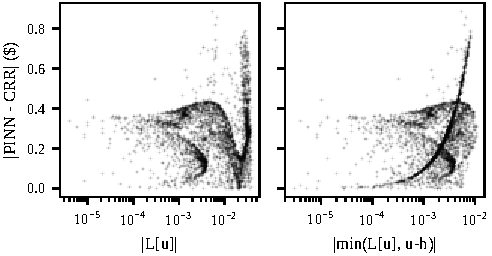
\includegraphics[width=\columnwidth]{figures/fig_p2_residual_vs_error.pdf}
\caption{N2, seed 0, 4000 pool points. Absolute price error against the raw residual $|L[u]|$ (left) and the LCP residual (right). The raw residual shows no trend with the error; the LCP residual rises with it mainly in the exercise region (the curved branch).}
\label{fig:resid}
\end{figure}

\begin{table}[t]
\caption{Conformal bands, $n_{\mathrm{cal}}=800$, $n_{\mathrm{test}}=2000$, mean over 10 seeds $\times$ 20 splits. Width in \usd. Seed-to-seed std of coverage is at most \maxcovstd{}.}
\label{tab:conf}
\centering\footnotesize\setlength{\tabcolsep}{2.6pt}
\begin{tabular}{llrrrrrr}
\toprule
 & & \multicolumn{3}{c}{$\alpha=0.10$} & \multicolumn{3}{c}{$\alpha=0.05$}\\
Model & Score & Cov. & Width & Worst & Cov. & Width & Worst\\
\midrule
\tabinput{tables/table3_conformal.tex}
\bottomrule
\end{tabular}
\end{table}

\subsection{Conformal bands on PINN pricers}
Table~\ref{tab:conf} gives the main result. Marginal coverage is at its nominal level for every model and score, within 0.005. This also held for N2 before we fixed its bias. The finite-sample guarantee did its job, and the bias showed up as width (split band \usd 10.05). The PDE term shrinks the split band from \usd 19.43 (N0) to \usd 0.94 (N1) at $\alpha=0.10$, about 20 times. The choice of difficulty score matters. Normalising by $|L[u]|$ widens the N1 band (\usd 1.18 against \usd 0.94) and the N2 band (\usd 1.97 against \usd 0.93). It helps only N0, whose residual is large where it fails. For N2, the LCP residual narrows the band against $|L[u]|$ (\usd 1.13 against \usd 1.97) but not against split (\usd 0.93), and its worst bucket (0.64) is below split's (0.66). Mondrian gives the narrowest bands and the best worst-bucket coverage (0.86 against 0.66 for split on N2). Fig.~\ref{fig:bucket} shows that split under-covers deep in-the-money short tenors (0.69) and over-covers near-the-money long tenors (0.999), while Mondrian keeps each bucket between 0.901 and 0.906 on average. Fig.~\ref{fig:slice} shows the bands on one slice: they contain the reference and stay close to it, but the lower edges fall below zero far out of the money.

\begin{figure}[t]
\centering
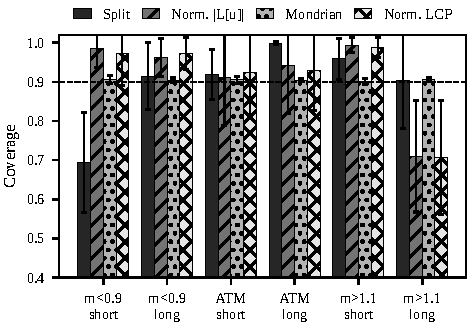
\includegraphics[width=\columnwidth]{figures/fig_p2_bucket_coverage_a10.pdf}
\caption{N2, $\alpha=0.10$, $n_{\mathrm{cal}}=800$: coverage per moneyness and tenor bucket (short: $\tau<0.4$), mean and std over 10 seeds. Dashed line: target 0.90. Only Mondrian is close to target in every bucket.}
\label{fig:bucket}
\end{figure}

\begin{figure}[t]
\centering
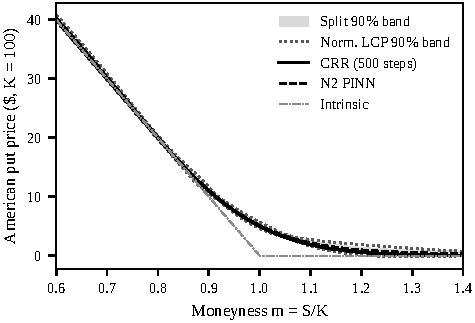
\includegraphics[width=\columnwidth]{figures/fig_p2_interval_slice_tau050.pdf}
\caption{American put at $\tau=0.5$, seed 0, $\alpha=0.10$. The split band (grey) and the LCP-normalised band (dotted) both contain the binomial price. The PINN lies slightly above it, most visibly out of the money, and the lower edges fall below zero far out of the money.}
\label{fig:slice}
\end{figure}

\subsection{Synthetic heteroscedastic check}
To isolate the score, we reuse a synthetic set with a known mean, noise standard deviation $0.01+0.12|m-1|$, difficulty $|m-1|$, $n_{\mathrm{cal}}=800$, $n_{\mathrm{test}}=2500$ and 50 seeds (Table~\ref{tab:p3}). Normalisation narrows the band (0.127 against 0.145 at $\alpha=0.10$) and raises coverage far from the money from 0.813 to 0.854. The fitted $\kappa$ is \kappafit{}, while the true ratio of slope to intercept is 12, so the adaptation is only partial. With homoscedastic noise, split coverage is 0.903 ($\alpha=0.10$) and 0.953 ($\alpha=0.05$).

\begin{table}[t]
\caption{Synthetic heteroscedastic data, 50 seeds. Width in $u$ units. Near: $|m-1|\le0.25$; far: $|m-1|>0.25$.}
\label{tab:p3}
\centering\footnotesize\setlength{\tabcolsep}{3.5pt}
\begin{tabular}{llrrrr}
\toprule
$\alpha$ & Score & Cov. & Width & Near & Far\\
\midrule
\tabinput{tables/table4_p3.tex}
\bottomrule
\end{tabular}
\end{table}

\subsection{Static arbitrage of prices and band edges}
We run the project's arbitrage checker on a put chain with $S=100$, strikes 60 to 140 in steps of 2.5 and ten expiries from 0.1 to 1 year, with tolerance $10^{-6}$ (Table~\ref{tab:p4}). Bands come from split 0, $n_{\mathrm{cal}}=800$, $\alpha=0.10$. The PINN prices break strike convexity in 12\% of checkable triples for both N1 and N2. The N2 point prices also break the calendar check in 16.8\% of pairs, and 2.4\% of these prices are negative. A constant split band keeps the convexity and calendar rates of the point price, since it only adds a term linear in $K$, but its lower edge raises monotonicity violations from 0.039 to 0.053. Bands of varying width add violations. About a fifth of lower edges are negative. The calendar check is not a valid condition for European puts: the exact Black-Scholes chain fails it in 27\% of cases. We apply no repair.

\begin{table}[t]
\caption{Static-arbitrage violation rates on a synthetic put chain (mean of 10 seeds). Put-call parity is not applicable to a put-only chain.}
\label{tab:p4}
\centering\footnotesize\setlength{\tabcolsep}{3pt}
\begin{tabular}{lrrrr}
\toprule
Series & Monot. & Convex & Calendar & Price${<}0$\\
\midrule
\tabinput{tables/table5_p4.tex}
\bottomrule
\end{tabular}
\end{table}

\section{Discussion}
\emph{Why keep the PINN if it loses on MAE?} It needs no labels, and it degrades gently outside any labelled region, where kernel and polynomial ridge fail (Table~\ref{tab:base}). It also exposes a residual for free. With a conformal layer, even a biased PINN gives bands with valid marginal coverage. The cost of the bias is width, so a better PINN gives narrower bands at once, as N1 against N0 shows, and as N2 before and after its fix shows (\usd 10.05 against \usd 0.93).

\emph{Which residual?} The residual should measure distance from the conditions that define the solution. For a European option that is $L[u]=0$. For an American option it is the LCP (\ref{eq:lcp}), and $|L[u]|$ is not zero at the true solution in the exercise region. The LCP residual fixes this and is a better error proxy than $|L[u]|$. Once the bias is fixed, though, no residual scaling beats plain split on width, and Mondrian buckets give the most even coverage. The two ideas can be combined in future work.

\emph{The N2 bias.} Our first N2 overpriced by \usd 3.13 on average. We traced this to the complementarity penalty. Its product form $L[u](u-h)$ is tiny where $u-h$ is small, so a network with $L[u]>0$ in the continuation region paid almost nothing. We replaced it with $\min(L[u],u-h)$ at weight 10 and set the American value 1 at $m=0$. The boundary change alone barely moved the bias. We chose the fix on a separate validation grid, not on calibration or test points. The fixed N2 keeps a bias of +\usd 0.22, largest for deep out-of-the-money long tenors (+\usd 0.35). It breaks the calendar check more often than before, and it sits below intrinsic value by more than one cent on 11\% of pool points.

\emph{What the data cannot show.} The project holds one Yahoo Finance snapshot of 4054 quotes from 13 Aug 2026 for SPX, NDX, NVDA and AAPL. One snapshot cannot support a time-ordered calibration and test split, so we report no market coverage. Real quotes also carry bid-ask noise and are not exchangeable across dates.

\section{Conclusion}
We placed split, normalised and Mondrian conformal bands on European and American PINN pricers. Marginal coverage held for every model, both before and after we fixed a bias in the American PINN. The PDE loss shrank the European band about 20 times. With 3000 labels, most labelled regressors remain more accurate in-sample.

The difficulty score must match the problem. The raw PDE residual is a poor score for the American put. The complementarity residual is better, but Mondrian buckets are the most useful choice in practice. Future work will remove the calendar violations and obstacle slack of N2, build a dated market panel for real coverage tests, project band edges onto arbitrage-free prices, and put a band on the exercise boundary $S^*(\tau)$.

\section*{Acknowledgment}
Dr. Manish Kumar Tiwari supervised this project, and we thank him for his guidance. Use of AI: Grok Bot, an AI assistant, produced the experiment scripts, the figures and first drafts of every section. We checked, edited and verified all of it, and we are responsible for the content.

\bibliographystyle{IEEEtran}
\bibliography{references_ieeeabbrv}

\end{document}
